% !TEX root = Document.tex
%%
%%  Annexes.
%%
%%  Note: Ne pas modifier la ligne ci-dessous.
\addcontentsline{toc}{compteur}{ANNEXES}

\Annexe{VISUALISATION DES ÉTAPES DE L'ALGORITHME DE SUIVI DE MUR}
\label{annexe:suivi_mur}
\begin{tabular}{cc}
  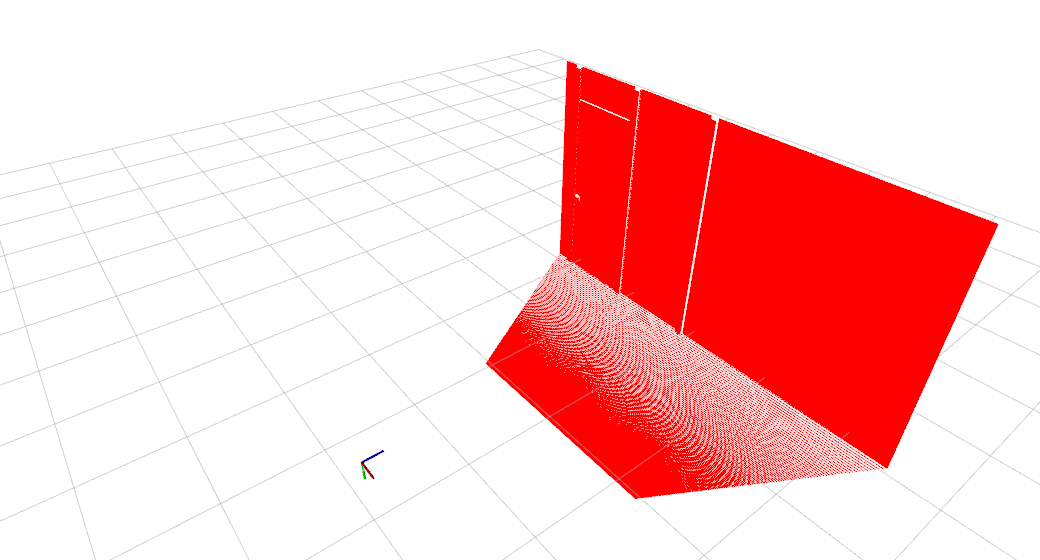
\includegraphics[width=0.5\linewidth]{images/pcl/Selection_060} &
  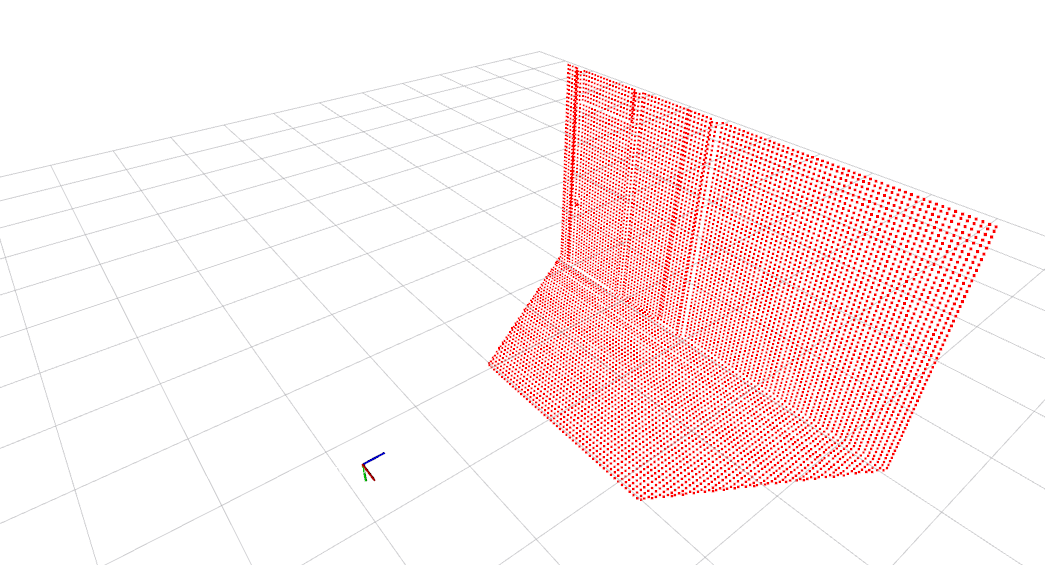
\includegraphics[width=0.5\linewidth]{images/pcl/Selection_061} \\
  (1) & (2) \\
  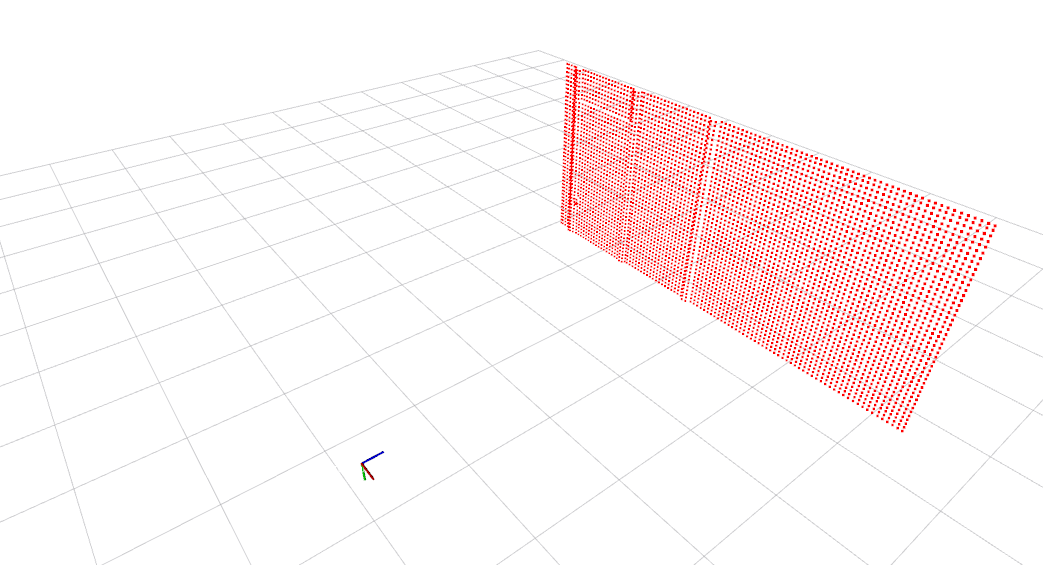
\includegraphics[width=0.5\linewidth]{images/pcl/Selection_062} &
  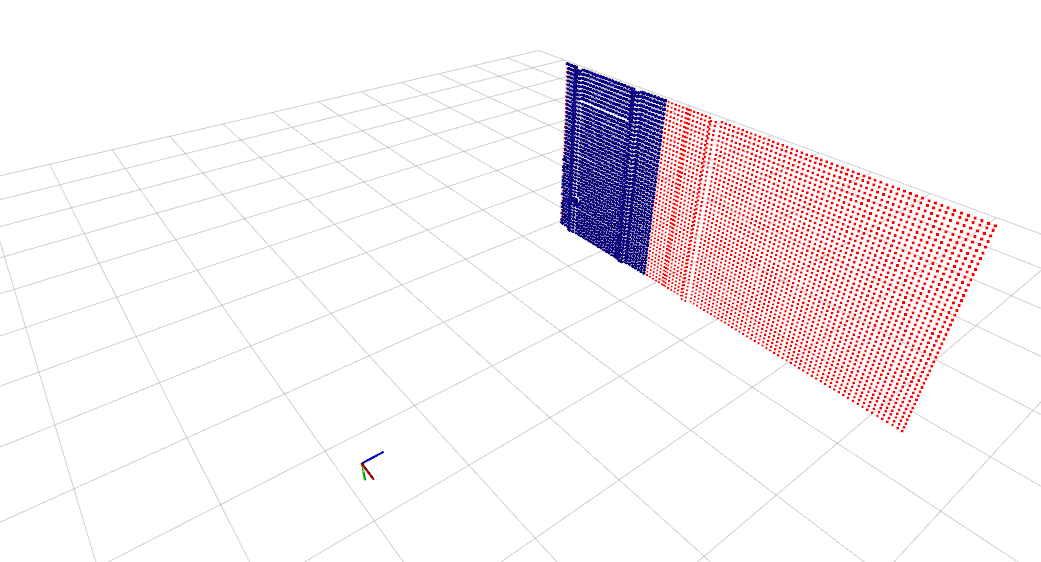
\includegraphics[width=0.5\linewidth]{images/pcl/Selection_063} \\
  (3) & (4) \\
  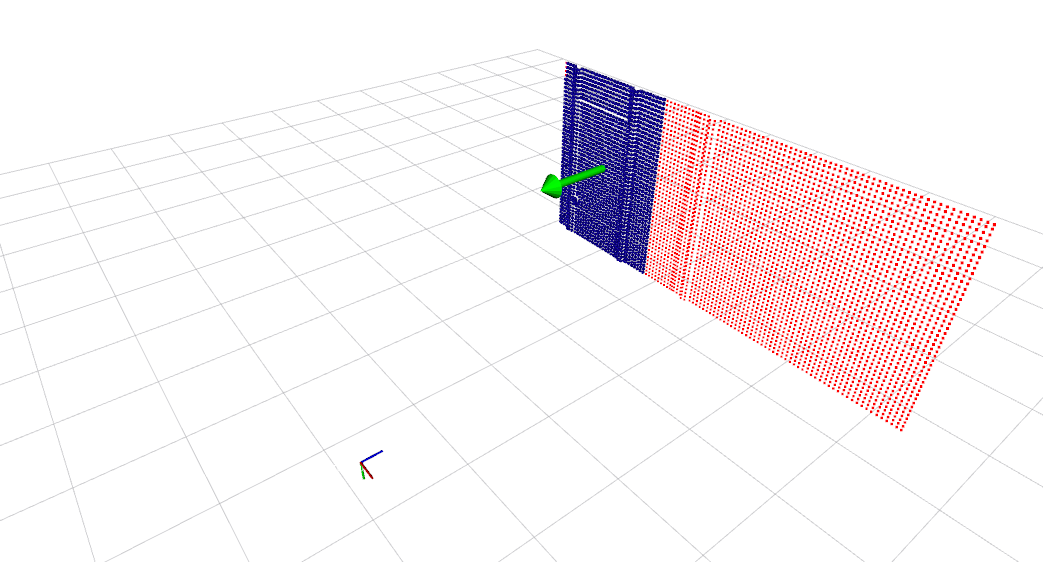
\includegraphics[width=0.5\linewidth]{images/pcl/Selection_064} &
  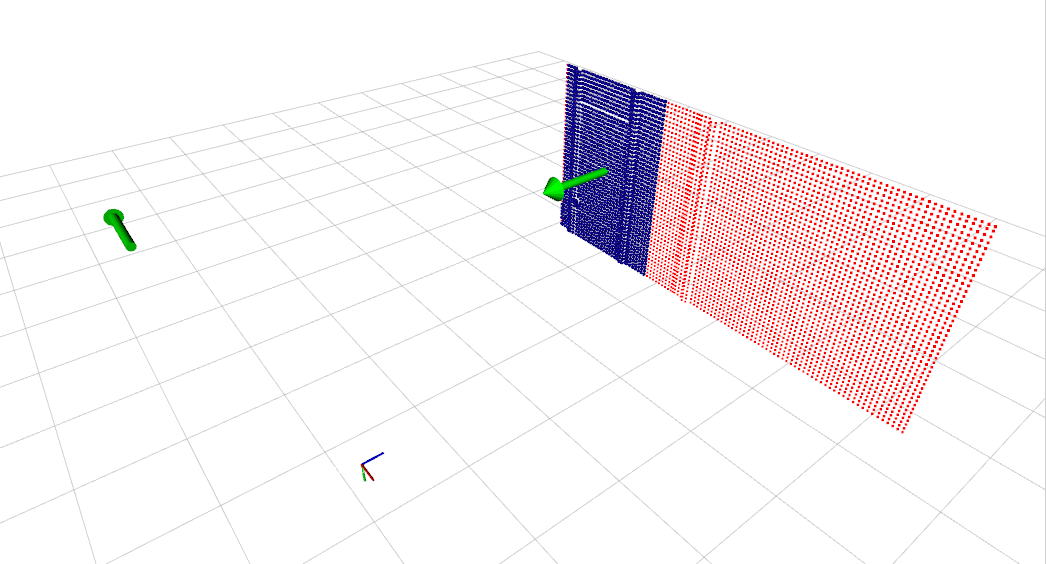
\includegraphics[width=0.5\linewidth]{images/pcl/Selection_065} \\
  (5) & (6)
\end{tabular}

(1) Nuage de points initial. (2) Downsampling du nuage. (3) Filtrage du sol par seuillage de la coordonnée $z$. (4) Sélection de un tiers du nuage vers l'avant du robot. (5) Calcul de la normale par ACP. (6) Calcul de la nouvelle pose objectif en prenant une longueur de pas dans la direction obtenue par le produit vectoriel entre la normale et l'axe $z$ du robot.

\Annexe{MACHINE À ÉTATS POUR L'INSPECTION D'ÉOLIENNES}
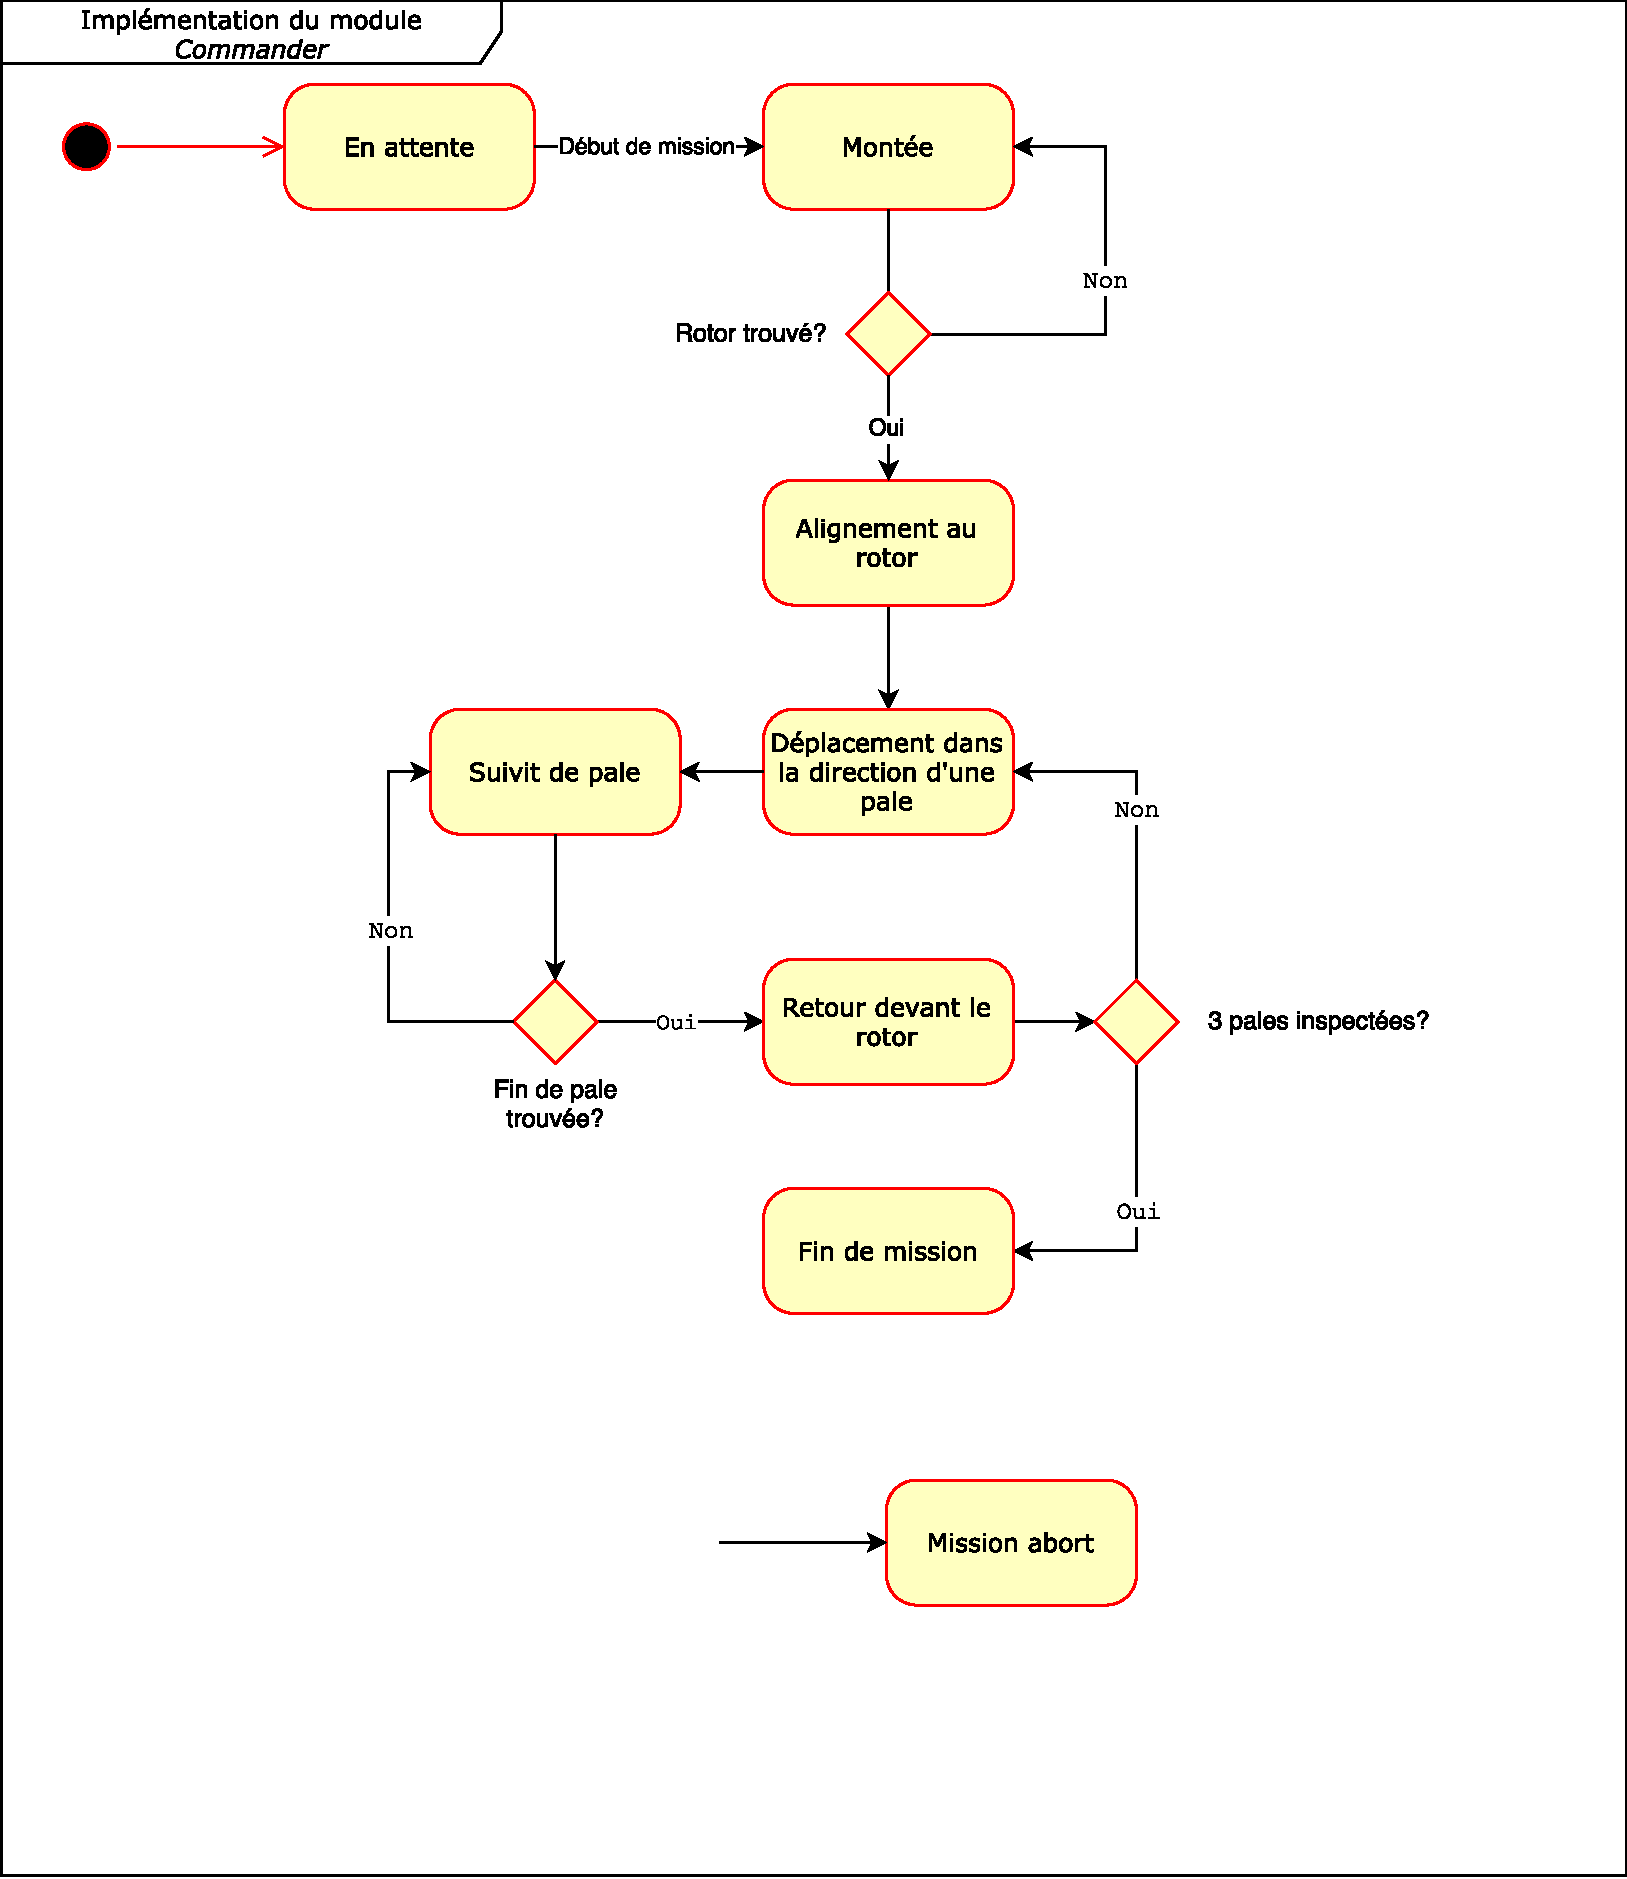
\includegraphics[width=\linewidth]{images/state_machine.pdf}
\label{annexe:state_machine}

\Annexe{LISTE DES PUBLICATIONS}
\begin{longtable}{lp{5in}}
  [Journal]     & A. Borowczyk, D.-T. Nguyen, \textbf{A. Phu-Van Nguyen}, D. Q. Nguyen, D. Saussié and J. Le Ny, \textit{Autonomous Landing of a Quadcopter on a High-Speed Ground Vehicle}. AIAA Journal of Guidance, Control and Dynamics, In Press, 2017.\\

  [Conférence]  & A. Borowczyk, D.-T. Nguyen, \textbf{A. Phu-Van Nguyen}, D. Q. Nguyen, D. Saussié and J. Le Ny, \textit{Autonomous Landing of a Multirotor Micro Air Vehicle on a High Velocity Ground Vehicle}. Proceedings of the IFAC World Congress, Toulouse, France, July 2017.\\

  [Journal]      & M. S. Ramanagopal, \textbf{A. Phu-Van Nguyen} and J. Le Ny, A Motion Planning Strategy for the Active Vision-Based Mapping of Ground-Level Structures. Accepted by Transactions on Automation Science and Engineering, November 2017.
\end{longtable}

Le travail des deux premières publications à propos de l'atterrissage d'un quadricoptère sur une voiture en mouvement a été réalisé dans le cadre de la participation du \textit{Mobile Robotics and Autonomous Systems Laboratory} au DJI Challenge lors des session d'hiver et d'été 2016. N'étant pas directement liées au présent mémoire, elles sont mentionnées ici car plusieurs des méthodes de contrôle de véhicule aérien et de traitement d'images ont été apprises lors de notre participation à cette compétition. Mon rôle spéficique dans ce projet était l'aide au traitement d'images pour la détection de la plateforme d'atterrissage et l'aide au niveau de l'implémentation du système en C++.

La dernière publication intitulée \textit{A Motion Planning Strategy for the Active Vision-Based Mapping of Ground-Level Structures} a été initialement soumise en février 2016 par M. S. Ramanagopal et J. Le Ny au journal \textit{Transactions on Automation Science and Engineering} (T-ASE). Lors du retour de l'évaluation par les pairs, il a été demandé entres autres d'ajouter un volet expérimental à l'article afin de prouver la validité des algorithmes développés dans l'article. C'est à ce moment, lors de la session d'automne 2016 et au début de la session d'hiver 2017 que je me suis ajouté au projet pour faire l'implémentation sur un robot physique. Au moment de l'écriture du présent mémoire, l'article a été accepté pour publication dans une édition future du journal T-ASE. Nous présentons le travail réalisé dans le cadre de ce projet au Chapitre \ref{sec:ugv}.


%%  Toutes les annexes doivent être inclues dans ce document
%%  les unes à la suite des autres.
% \Annexe{DÉMO}
% Texte de l'annexe A\@. Remarquez que la phrase précédente se termine
% par une lettre majuscule suivie d'un point. On indique explicitement
% cette situation à \LaTeX{} afin que ce dernier ajuste correctement
% l'espacement entre le point final de la phrase et le début de la
% phrase suivante.


%\begin{landscape}
%\Annexe{ENCORE UNE ANNEXE}
%Texte de l'annexe B\@ en mode «landscape».
%\end{landscape}
%
%\Annexe{UNE DERNIÈRE ANNEXE}
%Texte de l'annexe C\@.
